\documentclass[a4paper]{article}
\usepackage[a4paper, margin=1in]{geometry}
% Some basic packages
\usepackage[utf8]{inputenc}
\usepackage[T1]{fontenc}
\usepackage{textcomp}
\usepackage[dutch]{babel}
\usepackage{url}
\usepackage{graphicx}
\usepackage{float}
\usepackage{booktabs}
\usepackage{enumitem}

\pdfminorversion=7

% Don't indent paragraphs, leave some space between them
\usepackage{parskip}

% Hide page number when page is empty
\usepackage{emptypage}
\usepackage{subcaption}
\usepackage{multicol}
\usepackage{xcolor}

% Other font I sometimes use.
% \usepackage{cmbright}

% Math stuff
\usepackage{amsmath, amsfonts, mathtools, amsthm, amssymb}
% Fancy script capitals
\usepackage{mathrsfs}
\usepackage{cancel}
% Bold math
\usepackage{bm}
% Some shortcuts
\newcommand\N{\ensuremath{\mathbb{N}}}
\newcommand\R{\ensuremath{\mathbb{R}}}
\newcommand\Z{\ensuremath{\mathbb{Z}}}
\renewcommand\O{\ensuremath{\emptyset}}
\newcommand\Q{\ensuremath{\mathbb{Q}}}
\newcommand\C{\ensuremath{\mathbb{C}}}

% Easily typeset systems of equations (French package)
\usepackage{systeme}

% Put x \to \infty below \lim
\let\svlim\lim\def\lim{\svlim\limits}

%Make implies and impliedby shorter
\let\implies\Rightarrow
\let\impliedby\Leftarrow
\let\iff\Leftrightarrow
\let\epsilon\varepsilon

% Add \contra symbol to denote contradiction
\usepackage{stmaryrd} % for \lightning
\newcommand\contra{\scalebox{1.5}{$\lightning$}}

% \let\phi\varphi

% Command for short corrections
% Usage: 1+1=\correct{3}{2}

\definecolor{correct}{HTML}{009900}
\newcommand\correct[2]{\ensuremath{\:}{\color{red}{#1}}\ensuremath{\to }{\color{correct}{#2}}\ensuremath{\:}}
\newcommand\green[1]{{\color{correct}{#1}}}

% horizontal rule
\newcommand\hr{
    \noindent\rule[0.5ex]{\linewidth}{0.5pt}
}

% hide parts
\newcommand\hide[1]{}

% si unitx
\usepackage{siunitx}
\sisetup{locale = FR}

% Environments
\makeatother
% For box around Definition, Theorem, \ldots
\usepackage{mdframed}
\mdfsetup{skipabove=1em,skipbelow=0em}
\theoremstyle{definition}
\newmdtheoremenv[nobreak=true]{definitie}{Definitie}
\newmdtheoremenv[nobreak=true]{eigenschap}{Eigenschap}
\newmdtheoremenv[nobreak=true]{gevolg}{Gevolg}
\newmdtheoremenv[nobreak=true]{lemma}{Lemma}
\newmdtheoremenv[nobreak=true]{propositie}{Propositie}
\newmdtheoremenv[nobreak=true]{stelling}{Stelling}
\newmdtheoremenv[nobreak=true]{wet}{Wet}
\newmdtheoremenv[nobreak=true]{postulaat}{Postulaat}
\newmdtheoremenv{conclusie}{Conclusie}
\newmdtheoremenv{toemaatje}{Toemaatje}
\newmdtheoremenv{vermoeden}{Vermoeden}
\newtheorem*{herhaling}{Herhaling}
\newtheorem*{intermezzo}{Intermezzo}
\newtheorem*{notatie}{Notatie}
\newtheorem*{observatie}{Observatie}
\newtheorem*{oef}{Oefening}
\newtheorem*{opmerking}{Opmerking}
\newtheorem*{praktisch}{Praktisch}
\newtheorem*{probleem}{Probleem}
\newtheorem*{terminologie}{Terminologie}
\newtheorem*{toepassing}{Toepassing}
\newtheorem*{uovt}{UOVT}
\newtheorem*{vb}{Voorbeeld}
\newtheorem*{vraag}{Vraag}

\newmdtheoremenv[nobreak=true]{definition}{Definition}
\newtheorem*{eg}{Example}
\newtheorem*{notation}{Notation}
\newtheorem*{previouslyseen}{As previously seen}
\newtheorem*{remark}{Remark}
\newtheorem*{note}{Note}
\newtheorem*{problem}{Problem}
\newtheorem*{observe}{Observe}
\newtheorem*{property}{Property}
\newtheorem*{intuition}{Intuition}
\newmdtheoremenv[nobreak=true]{prop}{Proposition}
\newmdtheoremenv[nobreak=true]{theorem}{Theorem}
\newmdtheoremenv[nobreak=true]{corollary}{Corollary}

% End example and intermezzo environments with a small diamond (just like proof
% environments end with a small square)
\usepackage{etoolbox}
\AtEndEnvironment{vb}{\null\hfill$\diamond$}%
\AtEndEnvironment{intermezzo}{\null\hfill$\diamond$}%
% \AtEndEnvironment{opmerking}{\null\hfill$\diamond$}%

% Fix some spacing
% http://tex.stackexchange.com/questions/22119/how-can-i-change-the-spacing-before-theorems-with-amsthm
\makeatletter
\def\thm@space@setup{%
  \thm@preskip=\parskip \thm@postskip=0pt
}


% Exercise 
% Usage:
% \oefening{5}
% \suboefening{1}
% \suboefening{2}
% \suboefening{3}
% gives
% Oefening 5
%   Oefening 5.1
%   Oefening 5.2
%   Oefening 5.3
\newcommand{\oefening}[1]{%
    \def\@oefening{#1}%
    \subsection*{Oefening #1}
}

\newcommand{\suboefening}[1]{%
    \subsubsection*{Oefening \@oefening.#1}
}


% \lecture starts a new lecture (les in dutch)
%
% Usage:
% \lecture{1}{di 12 feb 2019 16:00}{Inleiding}
%
% This adds a section heading with the number / title of the lecture and a
% margin paragraph with the date.

% I use \dateparts here to hide the year (2019). This way, I can easily parse
% the date of each lecture unambiguously while still having a human-friendly
% short format printed to the pdf.

\usepackage{xifthen}
\def\testdateparts#1{\dateparts#1\relax}
\def\dateparts#1 #2 #3 #4 #5\relax{
    \marginpar{\small\textsf{\mbox{#1 #2 #3 #5}}}
}

\def\@lecture{}%
\newcommand{\lecture}[3]{
    \ifthenelse{\isempty{#3}}{%
        \def\@lecture{Lecture #1}%
    }{%
        \def\@lecture{Lecture #1: #3}%
    }%
    \subsection*{\@lecture}
    \marginpar{\small\textsf{\mbox{#2}}}
}



% These are the fancy headers
\usepackage{fancyhdr}
\pagestyle{fancy}

% LE: left even
% RO: right odd
% CE, CO: center even, center odd
% My name for when I print my lecture notes to use for an open book exam.
% \fancyhead[LE,RO]{Gilles Castel}

\fancyhead[RO,LE]{\@lecture} % Right odd,  Left even
\fancyhead[RE,LO]{}          % Right even, Left odd

\fancyfoot[RO,LE]{\thepage}  % Right odd,  Left even
\fancyfoot[RE,LO]{}          % Right even, Left odd
\fancyfoot[C]{\leftmark}     % Center

\makeatother




% Todonotes and inline notes in fancy boxes
\usepackage{todonotes}
\usepackage{tcolorbox}

% Make boxes breakable
\tcbuselibrary{breakable}

% Verbetering is correction in Dutch
% Usage: 
% \begin{verbetering}
%     Lorem ipsum dolor sit amet, consetetur sadipscing elitr, sed diam nonumy eirmod
%     tempor invidunt ut labore et dolore magna aliquyam erat, sed diam voluptua. At
%     vero eos et accusam et justo duo dolores et ea rebum. Stet clita kasd gubergren,
%     no sea takimata sanctus est Lorem ipsum dolor sit amet.
% \end{verbetering}
\newenvironment{verbetering}{\begin{tcolorbox}[
    arc=0mm,
    colback=white,
    colframe=green!60!black,
    title=Opmerking,
    fonttitle=\sffamily,
    breakable
]}{\end{tcolorbox}}

% Noot is note in Dutch. Same as 'verbetering' but color of box is different
\newenvironment{noot}[1]{\begin{tcolorbox}[
    arc=0mm,
    colback=white,
    colframe=white!60!black,
    title=#1,
    fonttitle=\sffamily,
    breakable
]}{\end{tcolorbox}}




% Figure support as explained in my blog post.
\usepackage{import}
\usepackage{xifthen}
\usepackage{pdfpages}
\usepackage{transparent}
\newcommand{\incfig}[1]{%
    \def\svgwidth{\columnwidth}
    \import{./figures/}{#1.pdf_tex}
}

% Fix some stuff
% %http://tex.stackexchange.com/questions/76273/multiple-pdfs-with-page-group-included-in-a-single-page-warning
\pdfsuppresswarningpagegroup=1

\title{\Huge{Probability}\\ Stationarity and Periodicity}
\author{\huge{Daniel Yu}}
\date{October 22, 2024}

\pdfsuppresswarningpagegroup=1

\begin{document}
\maketitle
\newpage% or \cleardoublepage
% \pdfbookmark[<level>]{<title>}{<dest>}
\tableofcontents
\pagebreak

\section{Stationary Distributions}
\begin{note}
  What is the long-term behavior of an absorbing markov chain? It gets absorbed by one of the absorbing states but which one? Thus, the question is: What is the probability that I get absorbed by any particular absorbing state in the markov chain?
\end{note}

\begin{theorem}
  $P[\text{ends at a} \mid X_0  = i] = \left( NR \right)_{i,a}  $ for any transient state $i$ and absorbing state  $a$. $N = (Q-I)^{-1}$ from the matrix    
  \[
     P = \begin{pmatrix} Q & R \\ 0 & I \end{pmatrix}
   .\]  

\noindent\hrulefill

\begin{proof}
   Let \( X_n \) denote the state of the chain at step \( n \) before absorption. We want to compute \( P[\text{absorbed at } a \mid X_0 = i] \) for an initial transient state \( i \) and absorbing state \( a \).

   By the law of total probability, we have:
   \begin{align*}
       P[\text{absorbed at } a \mid X_0 = i] &= \sum_{n=0}^{\infty} \sum_{j} P[\text{absorbed at } a \mid X_n = j, X_0 = i] \cdot P[X_n = j \mid X_0 = i].
   \end{align*}

   Since absorption is an absorbing event and the chain can be "reset" upon reaching any transient state \( j \), we focus on the probability of reaching \( a \) from \( j \) in one step after reaching \( j \) from \( i \) after \( n \) steps. For any transient \( j \), by the time-homogeneity of Markov chains, we get:
   \begin{align*}
       P[\text{absorbed at } a \mid X_n = j, X_0 = i] &= P[X_1 = a \mid X_0 = j].
   \end{align*}

   Therefore,
   \begin{align*}
       P[\text{absorbed at } a \mid X_0 = i] &= \sum_{n=0}^{\infty} \sum_{j} P[X_1 = a \mid X_0 = j] \cdot P[X_n = j \mid X_0 = i] \\
       &= \sum_{n=0}^{\infty} \sum_{j} R_{j,a} \cdot (Q^n)_{i,j} \\
       &= \sum_{j} R_{j,a} \sum_{n=0}^{\infty} (Q^n)_{i,j}.
   \end{align*}

   The inner sum \( \sum_{n=0}^{\infty} (Q^n)_{i,j} = (I + Q + Q^{2} + \ldots)_{i,j} \) represents the expected number of times the chain is in state \( j \) given it starts at \( i \), which is the \( (i,j) \)-entry of the fundamental matrix \( N = (I - Q)^{-1} \). Thus,
   \begin{align*}
       P[\text{absorbed at } a \mid X_0 = i] &= \sum_{j} R_{j,a} \cdot N_{i,j} \\
       &= (NR)_{i,a}.
   \end{align*}
   This completes the proof.
\end{proof}

 \end{theorem}

\begin{note}
  What is the long-term effect of non-absorbing time-homogenous markov chains?
\end{note}

\begin{definition}
  A pair of states $i \neq j$ are intercommunicating. if starting at $i$, I can make it to  $j$ and starting at  $j$, I can make it to  $i$. Formally  $i \equiv j$ (equivalence relation) if :
   \begin{align*}
     \exists n \text{ such that} P[X_n=j \mid  X_0 = i] > 0, \text{ i.e.} (P^{n})_{i,j} > 0 \\
     \exists m \text{ such that} P[X_m=i \mid  X_0 = j] > 0, \text{ i.e.} (P^{m})_{j,i} > 0
  .\end{align*}
\end{definition}

\begin{definition}
  Define $C_i = \{\text{ all states } j: i \equiv j  \} $. Trivially, each vertex (state) is an equivalent to itself, so the equivalence class of  $C_i$ must be nonempty.
\end{definition}

\begin{theorem}
  We can partition the state space $\Omega$ into \textbf{intercommunicating classes}  $\{C_i\} $ (i.e can partition the vertices of the graph into subgraphs) .   Note that this forms \textbf{strongly connected components}
\end{theorem}

\begin{definition}
  A markov chain is \textbf{irreducible} if it has precisely one intercommunicating class (i.e. $\forall i,j \in \Omega, \exists n$ such that $P[X_n =j \mid  X_0 =i] > 0, (P^{n})_{i,j} > 0$ )
\end{definition}

\begin{definition}
  A markov chain is \textbf{regular} if $\exists N$, a single choice, such that $\forall i,j, (P^{N})_{i,j} > 0$ which implies that $P[X_N = j \mid X_0=i] > 0$.    
\end{definition}

\begin{note}
  Not all markov chains that are irreducible are regular. For example, consider $P = \begin{pmatrix}  0 & 1\\ 1 & 0 \end{pmatrix}$ which is irreducible but not regular. There is no way to make all four entries strictly positive for one choice of $N$ in  $P^{N}$ \end{note}

\begin{theorem}
  if $i \equiv j$ then both are recurrent or both transient  
\end{theorem}


\begin{prop}
  If $\mid \Omega \mid  < \infty$ then at least one state is recurrent.

  \begin{proof} 
    Assume by contradiction that all states are transient. Then $V(i) < \infty$ $\forall i \in \Omega$. But  $\sum_{i \in \Omega} V(i) = \infty$ since we can continue the markov chain forever. This is a contradiction, so at least one $V(i) = \infty$ and thus recurrent.
  \end{proof}
\end{prop}

\begin{corollary}
  given the theorem and proposition, then all states in a irreducible markov chain are recurrent.
\end{corollary}

\begin{note}
\begin{enumerate}
  \item Given an irreducible Markov chain $\{X_n\} $, what proportion of time is spent in state $i$? Does the answer to the above matter depending on where I start?
  \item LEt $\{X_n\}_{n =0,1,2,\ldots} $ be the sequence of RV. Does $X_n$ converge in distribution? i.e. 
     \[
       \lim_{n \to \infty} P[X_n=j \mid X_0=i] \to c
    ?\] Does it depend on $X_0=i$?
\end{enumerate} 
\end{note}

\begin{definition}
  A row vector $\pi$ is \textbf{stationary} if  $\pi P = \pi$ and $\pi_{i} \geq 0$. Notice that this is equivalent to saying
  $\pi$ is a row-eigenvector of $P$ with  $\lambda = 1$.  So,
  \[
  \pi P^{n} = (\pi P) \times P \ldots \times P = \pi
  .\] 
\begin{remark}
  $\sum_{i=\Omega} \pi_i = 1$ blc probability
\end{remark}
\end{definition}

\begin{note}{Example}\\
  Suppose $\pi$ is stationary vector and $P[X_0 =j] = \pi_j$:
  \begin{align*}
    P[X_i=j] &= \sum_{i \in \Omega} P[X_i =j \mid X_0 =i] \cdot P[X_0 = i]\\
             &= \sum_{i \in \Omega} P_{i,j} \pi_j \\
             &= (\pi P)_{j} \\
             &= \pi_{j}
  .\end{align*}
\end{note}

\begin{note}{Only for irreducible markov chain}\\
  So if we have $X_0 \sim \pi$ (i.e.  $P[X_0=i] = \pi_i$, then the distribution of $X_n \sim \pi$). What if $X_0 \not\sim \pi?$
\end{note}

\noindent\hrulefill

\textbf{Intuition}
\begin{align*}
  P[X_n = j \mid  X_0 = i] &= (P^n)_{i,j} \\
                           &\text{We can diagonalize the matrix $P$, if it is diagonalizable, as: $P = Q \Lambda Q^{-1}$} \\
    &\text{where } \Lambda = \text{diag}(\lambda_1, \lambda_2, \ldots, \lambda_k) \text{ is a diagonal matrix with the eigenvalues of } P \\
    &= (Q \Lambda^n Q^{-1})_{i,j} \\
    & \text{Given that } \lambda_1 = 1 \text{ (1 is always an eigenvalue of a Markov transition matrix)} \\
    &\text{and for an irreducible Markov chain},\\
    &\text{the remaining eigenvalues satisfy } |\lambda_i| < 1 \text{ for } i \geq 2, \\
    &\text{as } n \to \infty, \Lambda^n = \text{diag}(1, \lambda_2^n, \lambda_3^n, \dots, \lambda_k^n) \to \text{diag}(1, 0, 0, \dots, 0), \\
    &= (Q \text{ diag}(1, 0, 0, \dots, 0) Q^{-1})_{i,j} \\
    &\approx \pi_j.
\end{align*}

\begin{theorem}
  Every finite-state markov chain has at least one stationary vector. If the finite state markov is irreducible this vector is unique.
\end{theorem}

\begin{lemma}
  Let $S$ be a row-stochastic matrix with strictly positive entries. 
   \[
  d = \min_{i,j} S_{i,j} > 0
  .\] 
  Let $v$ be a column vector, $M_0 = max \{v_i\} $, $m_0 = min \{v_i\} $. \\
  Let $M_1 = max \{(Sv)_{i}\}$, $m_1 = min \{(Sv)_{i}\} $ for all entries in  $Sv$.  Then,
  \[
  M_1 - m_1 \leq (1-2d) (M_0 - m_0)
  .\] 
  and $M_1 < m_0$ and $m_1 \gg m_0$.

  \noindent\hrulefill

  \begin{proof}
    \begin{align*}
      (Sv)_{i} &= \sum_{k \in \Omega} S_{i,k}\cdot v_k \\
               &\text{ to maximize this, let's assume $V_k = M_0$ for all  $k$ except one,  $V_{i^{*}} =m_0$ (worst case)} \\
               &\leq \left( \sum_{k \neq i^{*}} S_{i,k} \right)M_0 + S_{_{i, i^{*}}} m_0  
    .\end{align*}
    Since $S$ is positive and row stochastic matrix, the worst case scenario is  $\sum_{k \neq i^{*}} S_i,k = 1-d, S_{i,i^{*}} = d$. Thus, $\forall i$,
    \[
      (Sv)_{i} \leq (1-d)M_0 + d m_0
    .\] 


To bound \( m_1 \), assume \( v_k = m_0 \) for all \( k \neq i^* \), and \( v_{i^*} = M_0 \). Then, 
\[
(Sv)_i \geq \sum_{k \neq i^*} S_{i,k} m_0 + S_{i,i^*} M_0.
\]
Since \( \sum_{k \neq i^*} S_{i,k} = 1 - S_{i,i^*} = 1-d, S_{i,i^{*}}=d\),
\[
(Sv)_i \geq (1 - d) m_0 + d M_0.
\]

Combining the upper and lower bounds, we get:
\[
M_1 - m_1 \leq \left[ (1 - d) M_0 + d m_0 \right] - \left[ (1 - d) m_0 + d M_0 \right].
\]
Simplifying the expression:
\[
M_1 - m_1 \leq (1 - 2d)(M_0 - m_0).
\]

which implies that the range of the vector \( v \) shrinks by at least a factor of \( (1 - 2d) \) after each application of \( S \). Since \( 0 < d < 1/2 \), repeated application of \( S \) after $k$ steps leads to convergence toward a stationary vector where \( M_k = m_k \) i.e. max = min, proving contraction of the range. Therefore, the stationary distribution is unique.
  \end{proof}
\end{lemma}

\begin{corollary}
  Let $P$ be the transition matrix of a regular finite state markov chain. If  $Pv = v$ for some column vecetor  $v$, then  $v$ is constant. In particular,  $Null(P-I)=\vec{1}$. 

  \noindent\hrulefill

  \begin{proof}
$\exists N$ such that $P^N$ is strictly positive and row-stochastic. Let $M_0$ and $ m_0$ be the maximum and minimum of $v$, and let $M_1$ and $m_1$ be the maximum and minimum of $P^N v$. By the lemma, we have
\[
M_1 - m_1 \leq (1 - 2d)(M_0 - m_0).
\]
Since $P^N v = v$, it follows that $M_1 = M_0$ and $m_1 = m_0$. Therefore, from the inequality we conclude that
\[
M_0 - m_0 = 0,
\]
because $1 - 2d < 1$ and the only way for this inequality to hold is if $M_0 = m_0$.

Thus, the maximum and minimum values of $v$ are the same, implying that $v$ is a constant vector i.e. $v =\begin{pmatrix} x \\ \vdots\\x \end{pmatrix}$. Since for any $v'$, $Pv' = v'$  where $v'$ must be the constant vector, then in fact  $v' = cv$ and unique, the null space of $P - I$ is one-dimensional. Therefore, $Null(P - I) = \vec{1}$.
  \end{proof}
\end{corollary}

\begin{lemma}
  $dim(\pi) = 1$ for $\pi P = \pi$. If there exists a stationary vector for $P_1$, the transition matrix of a regular finite state markov chain, then the vector is unique.
\end{lemma}

\begin{theorem}{Ergodic Theorem}\\
  The ergodic theorem for finite state markov chain states the following. Let $P$ be a the transition matrix. Then $\lim_{n \to \infty} P^{n}$ exists, has constant columns, and each row is made up of the unique stationary vectors of $P$. Furthermore, for any intial probability distribution $v$,  $\lim_{n \to \infty} P^{n} v = \pi $ the unique stationary distribution.\\ 

  \noindent\hrulefill

   \begin{proof}
     Let $v_1$ be the first column of $P$ and let  $N$ be such taht  $P^{N}$ is strictly positive. Denote,
     \begin{align*}
       M_0 &= max \{v_1\} \\
       m_0 &= max \{v_1\} 
     .\end{align*}
     Let
     \begin{align*}
       M_k &= max \{P^{Nk} v_1\} \\
       m_k  &= min \{P^{Nk} v_1\}  
     .\end{align*}
     By the Lemma 1, $\{M_k\} $ is non-increasing sequence and $\{m_k\} $ is a non-descreasing sequence. We also know that $\left( M_k - m_k \right) \leq (1-2d) (M_0 - m_0) $. A limit must exists and we know that the convergence:
     \[
       \lim_{k \to \infty} m_k = \lim_{k \to \infty} M_k = w_1 \in [0,1]
     .\]
     and thus,
     \[
     \lim_{k\to \infty} \left( P^{Nk} v_1 \right) = \begin{pmatrix} w_1\\ \vdots\\ w_1 \end{pmatrix} 
     .\] 
     Now consider when $v$ is the  $j$th column vector of  $P$, dentoed as  $v_j$:
      \[
        \left( P^{NK} v_i \right) \to \begin{pmatrix} w_j\\ \vdots\\ w_j \end{pmatrix}
     .\] 
     So, 
     \[
     \lim_{n\to \infty} P^{n+1} = \lim_{n\to \infty} P^{n} (v_1, v_2, \ldots, v_{\mid \Omega \mid }) =  \begin{pmatrix}
w_1 & w_2 & \cdots & w_{|\Omega|} \\
w_1 & w_2 & \cdots & w_{|\Omega|} \\
\vdots & \vdots & \ddots & \vdots \\
w_1 & w_2 & \cdots & w_{|\Omega|}
\end{pmatrix}
     .\],
     all $w_i \geq 0$ and  $\sum_{i \in \Omega} w_i =1$ (since $P^{n}$ is still the transition matrix for markov chain).
     Only thing left is to show that $w = wP$ (and thus  $\pi = w$). Consider,
     \begin{align*}
       \lim_{n\to \infty} P^{n+1} &= \lim_{n\to \infty} P^{n} \cdot P \\
                                  &= \begin{pmatrix}
w_1 & w_2 & \cdots & w_{|\Omega|} \\
w_1 & w_2 & \cdots & w_{|\Omega|} \\
\vdots & \vdots & \ddots & \vdots \\
w_1 & w_2 & \cdots & w_{|\Omega|}
\end{pmatrix} \cdot P \\
                                  &= \begin{pmatrix}
w_1 & w_2 & \cdots & w_{|\Omega|} \\
w_1 & w_2 & \cdots & w_{|\Omega|} \\
\vdots & \vdots & \ddots & \vdots \\
w_1 & w_2 & \cdots & w_{|\Omega|}
\end{pmatrix} 
     .\end{align*}
  \end{proof}
  Consider any row, we get $\vec{w} = \vec{w} \cdot P$ and $\pi = w$
\end{theorem}

\begin{remark}
  It follows quite clearly that $\lim_{n \to \infty} (P^{n})_{i,j} = \lim_{n \to \infty} P[X_n = j \mid X_0 =i] = \pi_j$ the stationary distribution at $j$. If I suppose  $X_0 = i$, then $X_n \to \pi$ in distribution 
  \[
    \lim_{n \to \infty} P[X_n = j \mid X_0 = i] = \pi_j
  .\] 
\end{remark}

Geometrically, this is what is happening
\begin{figure}[h]
  \centering
  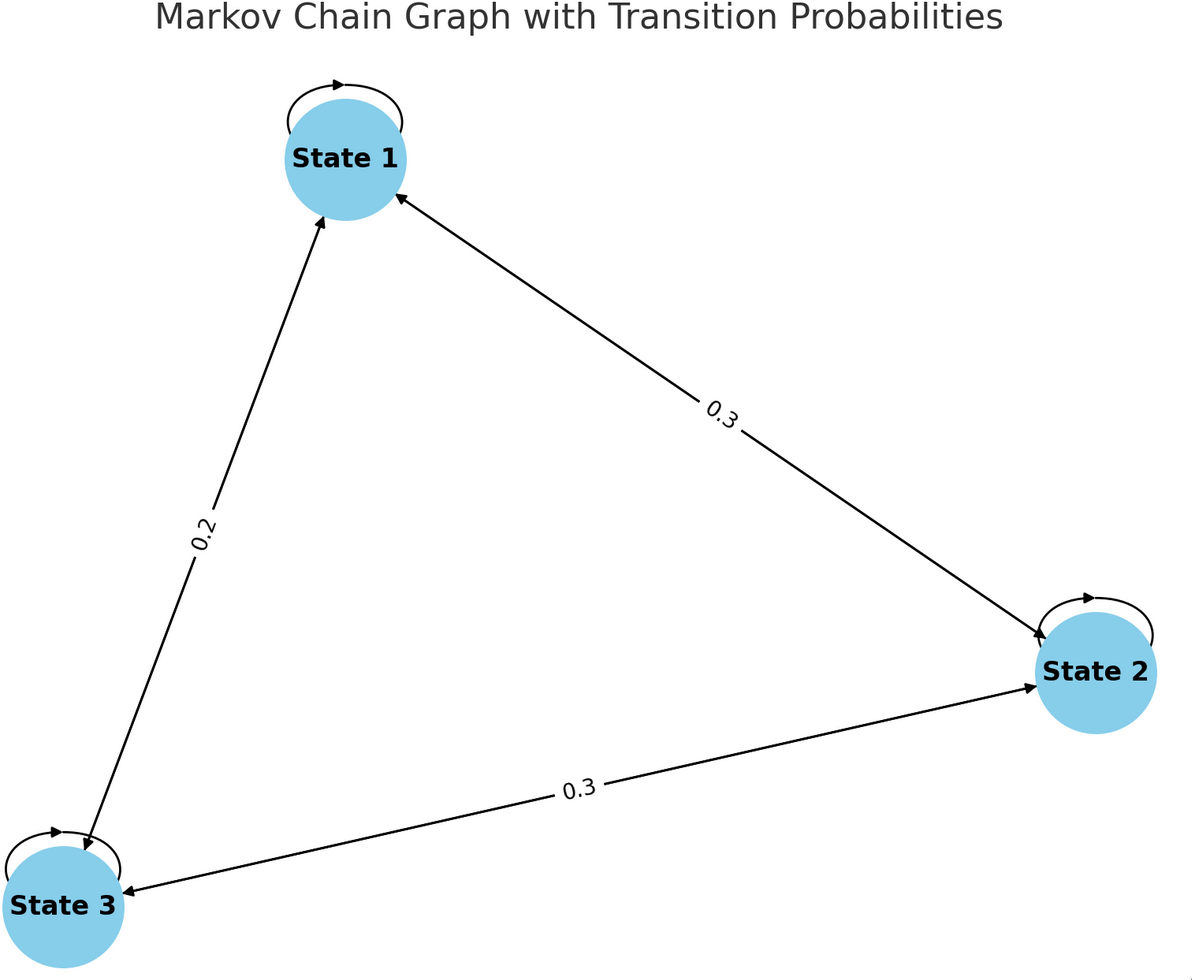
\includegraphics[width=0.8\textwidth]{assets/aperiodic_fs_markov_chain_ex.png}
  \caption{Markov Chain Example}
  \label{fig:aperiodic_fs_markov_chain_ex}
\end{figure}


\begin{figure}[H]
  \centering
  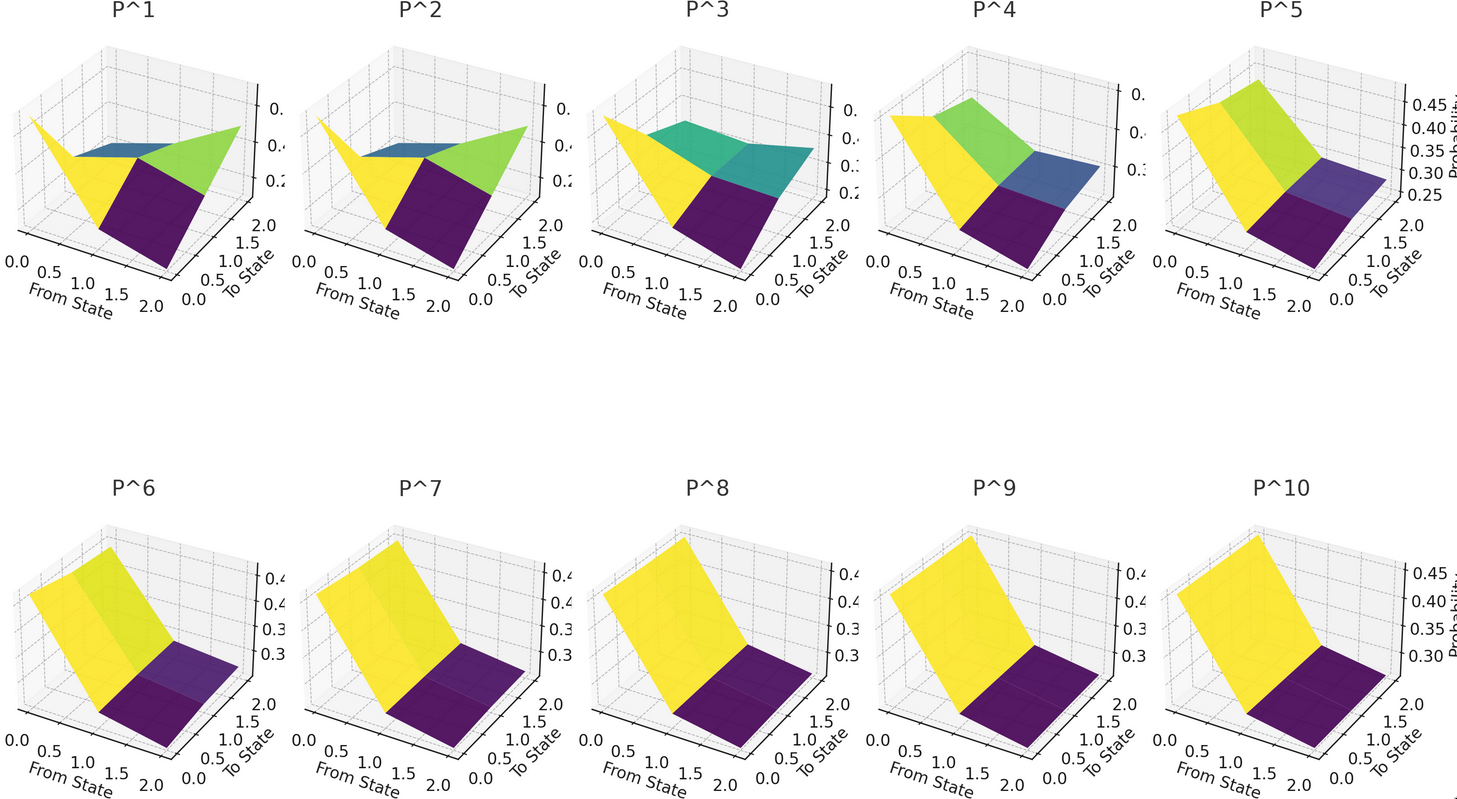
\includegraphics[width=0.8\textwidth]{assets/transition_matrix_convergence_stationary.png}
  \caption{Transition Matrix P converging to Stationary Distribution}
  \label{fig:transition_matrix_convergence_stationary}
\end{figure}

\begin{figure}[H]
  \centering
  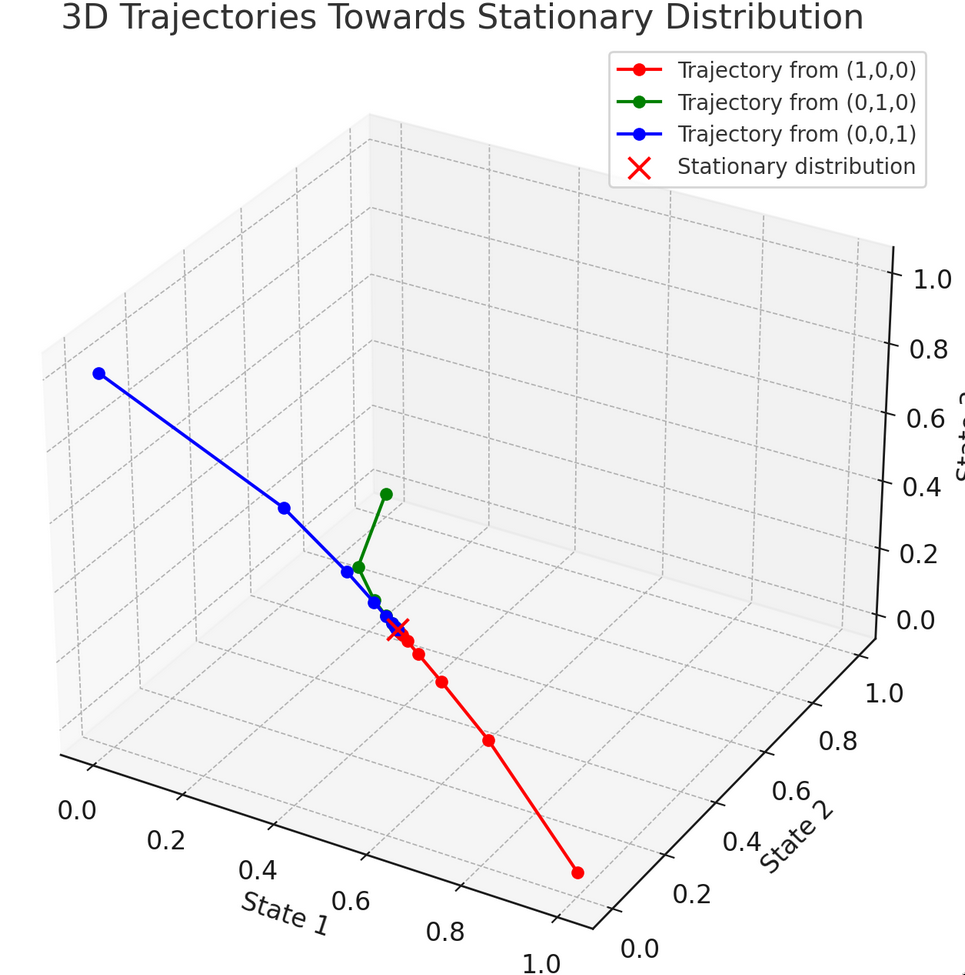
\includegraphics[width=0.8\textwidth]{assets/convergence_to_stationary_distribution.png}
  \caption{Trajectory of Convergence from starting vectors}
  \label{fig:convergence_to_stationary_distribution}
\end{figure}

\begin{theorem}
  For a state $i \in \Omega$, let  $F_n(j) = \frac{1}{n} \{\text{number of visits to $j$ up until time n}\}$. Let $V_k$ be the indicator variable  $V_k = 1\mid_{X_k = j}$. Then, $F_n(j) = \frac{1}{n} \sum_{k=1}^{n} V^{k}(j)$. We claim that 
   \[
  F_n (j) \to \pi_j
  .\] 
  in probabiltiy regardless of intial distribution.

  \begin{proof}
    To prove this we first need to compute:
    \begin{align*} 
      E[F_n(j) \mid X_0 =i] &= \frac{1}{n} \sum_{k=1}^{n} E[V^{k}\left( j \right) \mid X_0 =i] \\
                            &= \frac{1}{n} \sum_{k=1}^{n} P[X_k = j \mid X_0 =i] \\
                            &= \frac{1}{n} \sum_{k=1}^{n} (P^{k})_{i,j}
    .\end{align*}

  \end{proof}
\end{theorem}

\section{Periodicity}
Recall 
\begin{definition}
  A markov chain is \textbf{irreducible} if it has precisely one intercommunicating class (i.e. $\forall i,j \in \Omega, \exists n$ such that $P[X_n =j \mid  X_0 =i] > 0, (P^{n})_{i,j} > 0$ ).
\end{definition}

\begin{definition}
  A markov chain is regular if $\exists N$, a single choice, such that $\forall i,j, (P^{N})_{i,j} > 0$ which implies that $P[X_N = j \mid X_0=i] > 0$.    
\end{definition}

\begin{note}
  Notice the behavior for $P$,  $P^{N}_{1,1} > 0$ for $N$ even and $P^{N}_{1,2} > 0$ for $N$ odd. Can we describe this behavior?
\end{note}

\begin{definition}
  Thus, we introduce periodicity.
  \[
  S_i = \{n : P(X_n = i \mid X_0 = i) > 0\} 
  .\] 
  where the period is
  \[
    period(i) = gcd(S_i)
  .\]. A markov chain is \textbf{aperiodic} if $period(i) = 1 \forall i \in \Omega$  
\end{definition}

\begin{theorem}
 irreducible + regular $\implies$ aperiodic for finite state markov chains 
\end{theorem}

\begin{remark}
  Aperiodic, finite state markov chains are essentially \textbf{mixers}
\end{remark}

\end{document}
